\documentclass[../main.tex]{subfiles}

\begin{document}

In this chapter we introduce some preliminary concepts. 
Section \ref{AI-ML} introduce the early ideas in Artificial Intelligence and how they started advancements that led to state of the art methods.
Section \ref{ANN} introduce the Artificial Neural Network (ANN) model and how it is used in the Machine Learning context; we introduce the concept of Deep Learning and how Convolutional Neural Networks can be used to perform pattern recognition on images and spatially organized features. 
We also introduce the problem of deploying Deep Learnign models in resource constrained applications.
Sections \ref{ONNX} introduce the ONNX IR and why we need an intermediate representation for Deep Learning frameworks.

\newpage

\section{Artificial Intelligence and Machine Learning}
\label{AI-ML}

The Artificial Intelligence field is born in the 1950s with the goal of creating thought-capable artificial beings. 
With the creation of the computational model of the Turing machine the Computer Science field started studying how machine can act humanly and solve problems that were previously considered as exclusive domain of human intelligence.
Early efforts to create agents capable of showing intelligent behavior were directed toward creating decision-making algorithms, mostly focused on solving games with graph representations.
Even if first results were able to solve problems that were previously considered as unsolvable, the field soon realized that the approach was not well suited to solve different and more general problems.

Even if the early approaches were too general and failed to realize how complex the problem of creating a Artificial General Intelligence really is they sparked the emerging field of Machine Learning. 
The Computer Science field realized that the graph based approach lack the flexibility that is needed to create agents that show intelligent behavior; humans do not interact with their environment by optimizing a utility function and performing search algorithms in graph of possible states. 
Intelligent agents should be able to learn directly from the environment how to perform the computation needed to solve a specific problem.


The Machine Learning field changed the AI perspective by changing the paradigm of how the computation is performed. 
The program is not seen as given input of the system and the process is split into training and inference phases. 
The training phase use a set of sample data to learn how to perform a task without being explicitly programmed to solve it. 
The learned model must then be able to solve the same problem while being able to generalize on previously unseen samples.

\begin{figure}[h!]
    \centering
    \begin{subfigure}[]{0.4\textwidth}
        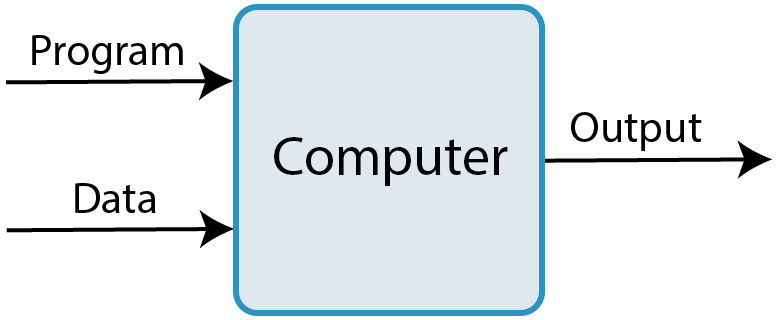
\includegraphics[width=\textwidth]{images/ML1.png}
        \caption{Traditional programming}
    \end{subfigure}
    \hspace{.1\linewidth}
    \begin{subfigure}[]{0.4\textwidth}
        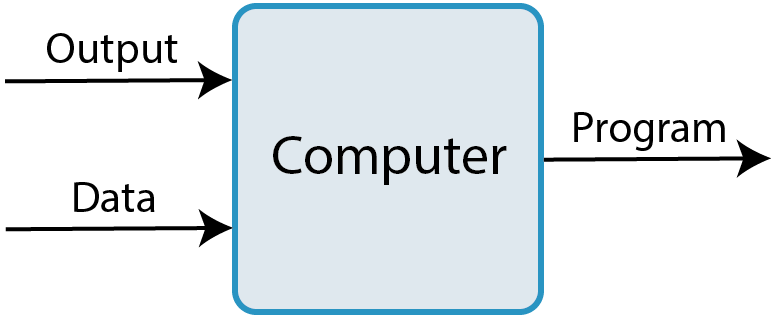
\includegraphics[width=\textwidth]{images/ML2.png}
        \caption{Machine Learning}
        \label{fig:ML2}
    \end{subfigure}
    \caption{ Comparison between the Traditional Programming approach and the Machine Learning approach}
    \label{fig:ML}
\end{figure}

Figure (a) show how the computation is usually performed in a traditional program execution; the computer produce the output by taking the program and the data as input. As comparison figure (b) show how the Machine Learning approach is fundamentally different. The program is not an input of the computer; the program is the output of the learning phase and is meant to be used to generalize on unseen data.

By splitting the process into training and inference phases the algorithm is able to learn a representation of the task to be used later as previous knowledge of the problem. 
Moreover, since the ML approach do not specify the kind of model that need to be used it can adapt by using the model that better fit a given task.

One of the most interesting models generated by the ML field is the Artificial Neural Network that is going to be presented in the next section.

\section{Artificial Neural Networks}
\label{ANN}

Artificial Neural Networks are powerful Machine Learning models inspired by how animal brains work.
ANNs are data driven models composed by artificial neurons and synapses that perform nonlinear transformations of input data.
In this section we present how ANNs work and how they evolved to solve more complex problems by using DL and CNN layers.

\subsection{Vanilla neural networks}
An Artificial Neural network is composed by multiple interconnected neurons. Each neuron is based on the perceptron model; a model invented in the 1950s with the goal of performing binary classification on input features.

\bigskip
\bigskip
\begin{figure}[h!]
  \centering
  %\subfigure{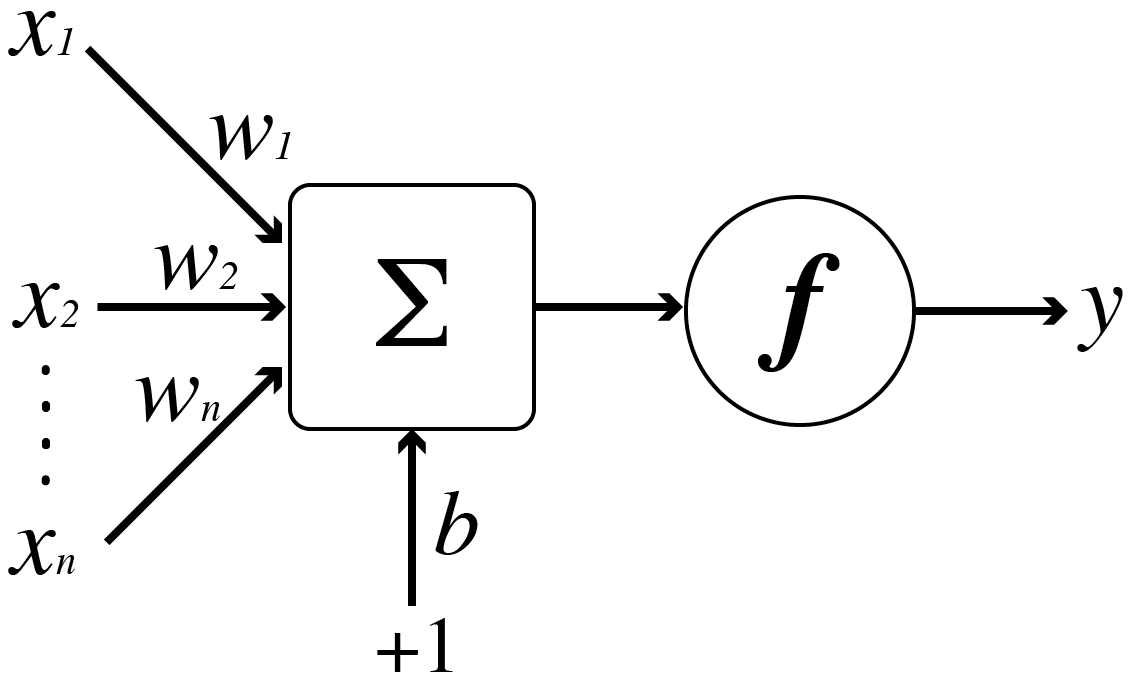
\includegraphics[width=.4\linewidth]{images/Perceptron.png}}
  %\subfigure{ $f(x) = x^2$ \vspace*{-20cm}}
  \begin{subfigure}[]{0.4\textwidth}
    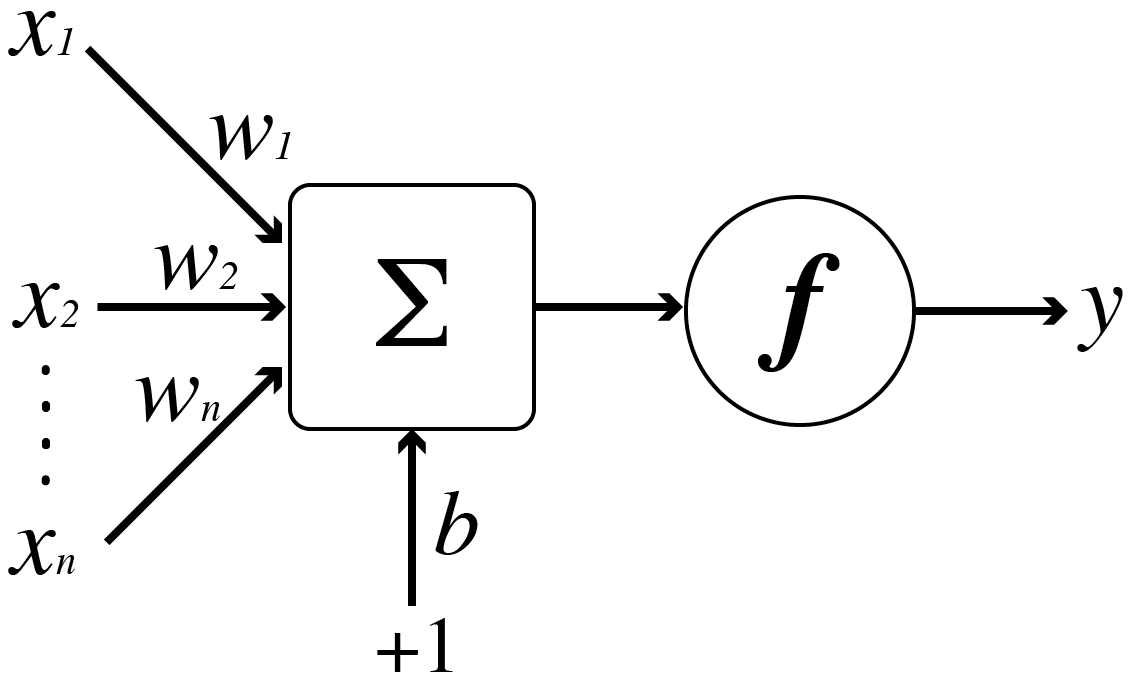
\includegraphics[width=\linewidth]{images/Perceptron.png}
  \end{subfigure}
  \begin{subfigure}[]{0.4\textwidth}
    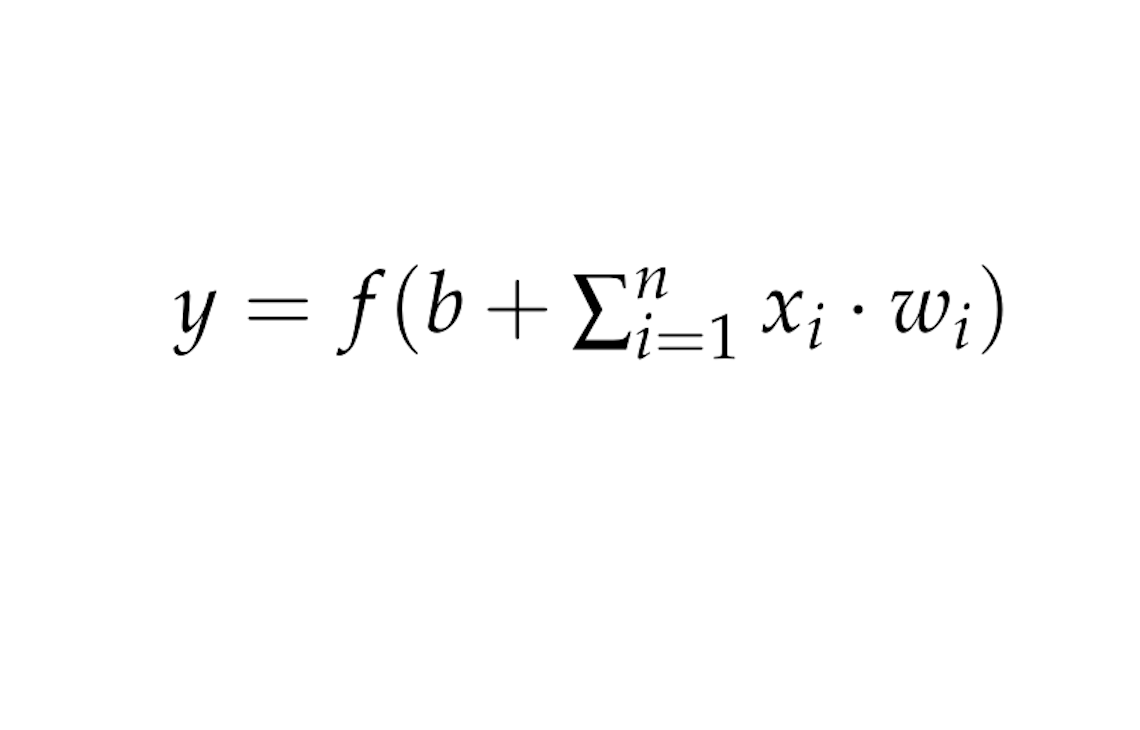
\includegraphics[width=\linewidth]{images/PerceptronFormula.png}
  \end{subfigure}
  \caption{Perceptron model}
  \label{fig:Perceptron}
\end{figure}

\newpage
To learn nonlinear representations of the input data the perceptron model use a nonlinear activation function before propagating the output value to the output connections. Two simple and common activation functions are the sigmoid and tanh functions.

\begin{figure}[h!]
    \centering
    \begin{subfigure}[]{0.4\textwidth}
        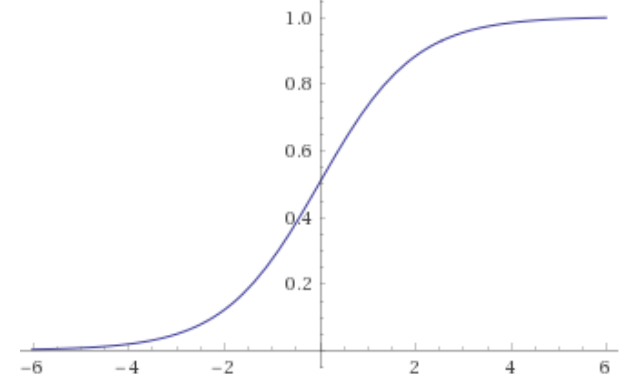
\includegraphics[width=\linewidth]{images/SigmoidFunction.png}
        \caption{$ {y = \frac{1}{(1+e^{-x})}} $}
        \label{fig:Sigmoid}
    \end{subfigure}
    \hspace{1cm}
    \begin{subfigure}[]{0.4\textwidth}
        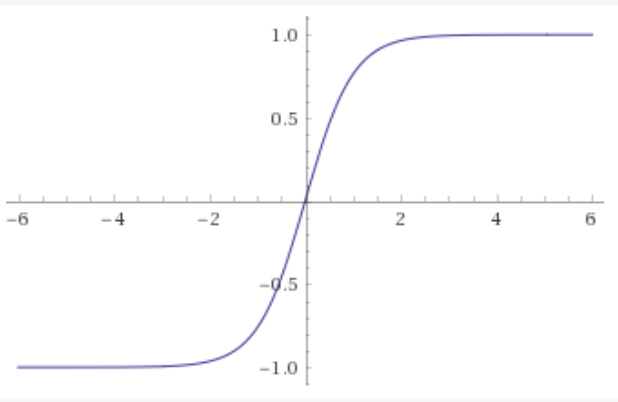
\includegraphics[width=\linewidth]{images/TanhFunction.png}
        \caption{$ {y = \tanh(x)} $}
        \label{fig:Tanh}
    \end{subfigure}
    \caption{Sigmoid (a) and Tanh (b) functions}
    \label{fig:SigmoidTanh}
\end{figure}


The perceptron model can be composed creating a network of interconnected neurons usally refered as Multi-Layer Perceptron.

\begin{figure}[h!]
  \centering
  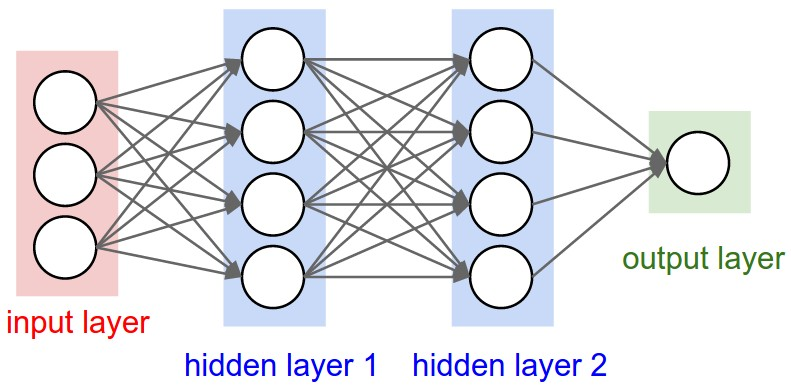
\includegraphics[width=.6\linewidth]{images/neural_net2.jpeg}
  \caption{Example of Multi-layer Perceptron network. \cite{CS231n}}
  \label{fig:MLP}
\end{figure}

The MLP model use a topology named Feed Forward configuration. 
A FF neural network is a MLP composed by a sequence of fully connected layers; a FF network always have one input and one output layer with a set of hidden layers in between.

Since the ANN model is computationally demanding and its use has been hold back by the limited computational resources availble, the use of the Feed Forward configuration is usually preferred to exploit SIMD instructions.
By seeing the network as a sequence of transformations over the input features, the algorithm can easily parallelize the training and inference phases on specialized HW by using SIMD instructions.
This allow the use of bigger and more complex networks leading to better performing models.


\subsection{ANN Training}
As previously stated a Machine Learning model need to be trained on a set of training data before being used with new and previously unseen samples.
The most common method to train a Neural Network is by means of supervised learning using the back-propagation algorithm.

The back-propagation algorithm is a gradient based optimization method.
Since the Neural Network is a differentiable model, given a differentiable function the back-propagation algorithm can calculate the network gradient (Also known as backward-pass) and iteratively optimize the network weights toward values corresponding to lower loss values.

The back-propagation algorithm is able to learn a set of weights that approximate the desired output, even in the case of Neural Networks with multiple hidden layers.
The weights belonging to hidden layers can not be directly calculated; the back-propagation algorithm need to use the chain rule to calculate the gradient of hidden layers.
This lead to the problem of the vanishing gradient.
Since the gradient vanishes while propagating through the layers this limit how deep a Neural Network can be. 
The gradient shrinks and layers distant to the output get trained more slowly than layers close to the output.

The problem is solved by using activation functions that do not shrink the gradient at each layer propagation.
As example we can use the ReLU activation function to avoid the problem.

\begin{figure}[h!]
    \centering
    \begin{subfigure}[c]{0.4\textwidth}
        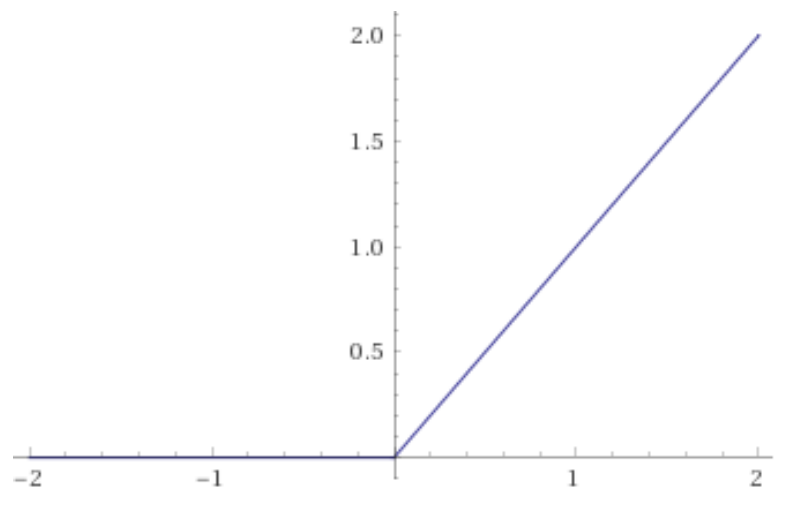
\includegraphics[width=\linewidth]{images/ReLU.png}
        \caption{$ {y = \max{(0,}{ x)}} $}
        \label{fig:ReLy}
    \end{subfigure}
    \hspace{1cm}
    \begin{subfigure}[c]{0.4\textwidth}
        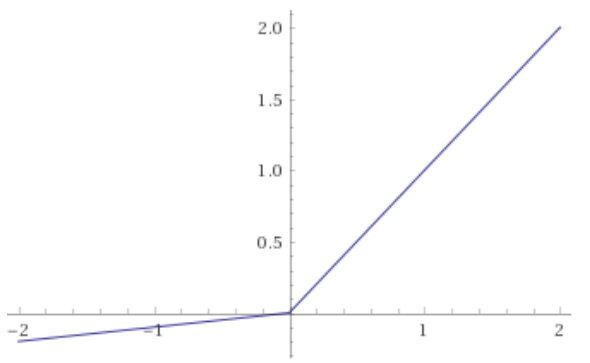
\includegraphics[width=\linewidth]{images/LeakyReLU.png}
        \caption{$ {y = } \left\{
            \begin{array}{ll}
                x & x\geq 0 \\
                ax & otherwise 
            \end{array} \right. $}
        \label{fig:LeakyReLU}
    \end{subfigure}
    \caption{Relu (a) and Leaky ReLU (b) functions.  }
    \label{fig:ReLUs}
\end{figure}

The ReLU function is introduced to avoid the problem of the vanishing gradient while being able to introduce a nonlinearity. Since the ReLU function have gradient equal to $0$ when $x\le 0$ most of the connections become deactivated during the training phase. To solve this problem multiple activation functions has been proposed; one example is the Leaky ReLU function that assign a small gradient $a\leq 1$ when $x$ is negative.

\subsection{Deep learning and Convolutitional Neural Networks}

The Artificial Neural Networks are powerful models to process high dimensional features but there are situations where the MLP model would require too many parameters to find a good approximation. To make an example in spatially organized data, such as images and sequence of words, the amount of weights that a MLP would require to find a good model would be intractable.

The term Deep Learning is often used to refer to the state of the art NN models that use different type of layers to tailor the model to the type of task that the network is supposed to learn.
DL models can use layers specifically designed to analyze sequences of data by using LSTMs and Attention layers. 
Other kinds of networks can use convolutional layers to extract features among spatially organized data such as 2D convolutions for images and 3D convolutions for videos.

In the field of Computer Vision a convolution operation is a well known operation used to extract interesting features in an image. 

The equation to compute a convolution on an image I and a kernel h is
\begin{equation}
 G(r,c) = (I \circledast h)(r,c) = \sum_{u=-L}^L \sum_{v=-L}^{L} I(r+u,c+v) \cdot h(-u, -v)
\end{equation}

For example when performing the edge detection the Canny edge detection algorithm use convolution operations to smooth the input image and detect the gradient wrt the x and y coordinates of the image. 


\begin{figure}[h!]
    \centering
    \begin{subfigure}[]{0.35\linewidth}
        \label{fig:CameramanSub}
        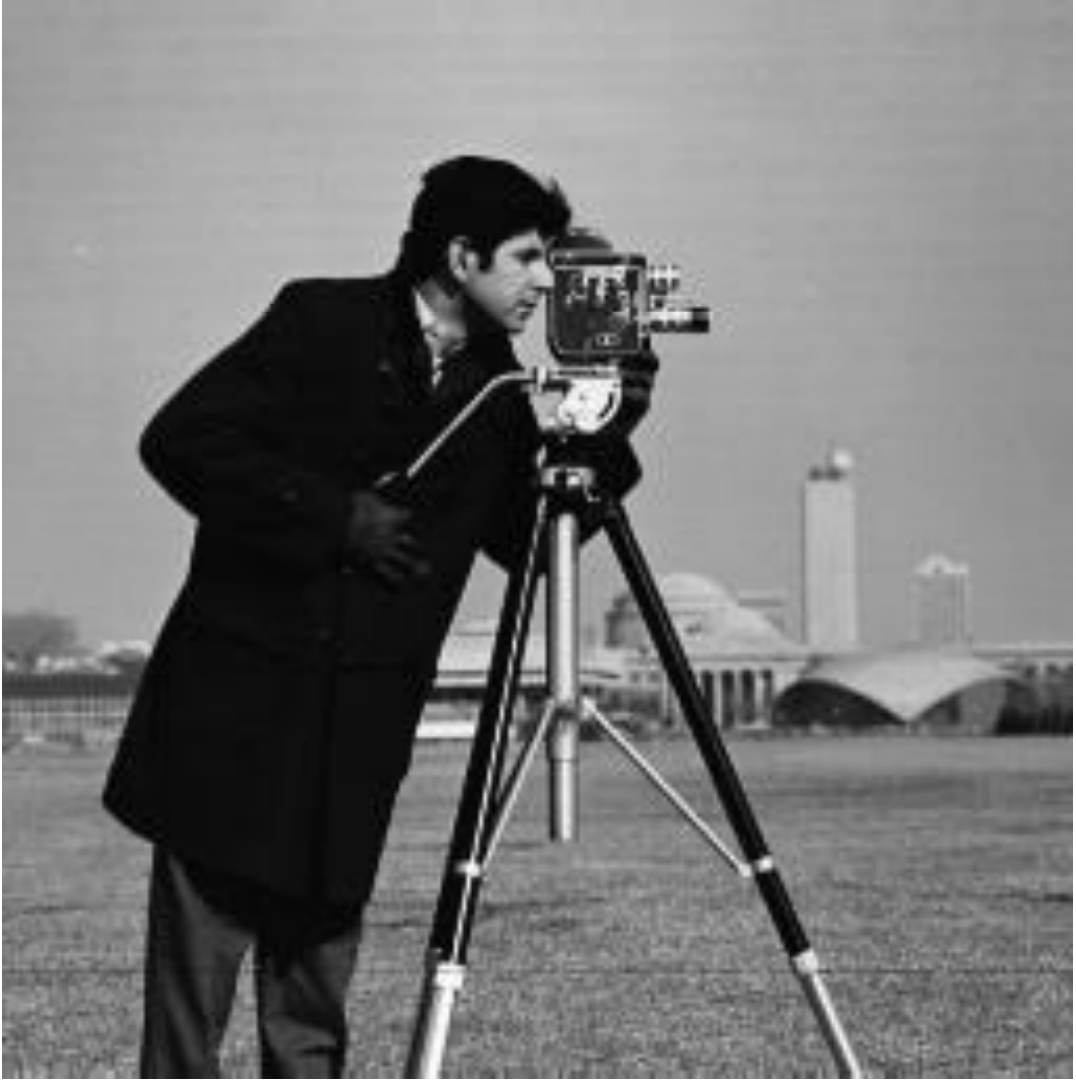
\includegraphics[width=\linewidth]{images/Cameraman.png}
    \end{subfigure}
    \hspace{1cm}
    \begin{subfigure}[]{.35\linewidth}
        \label{fig:CameramanDx}
        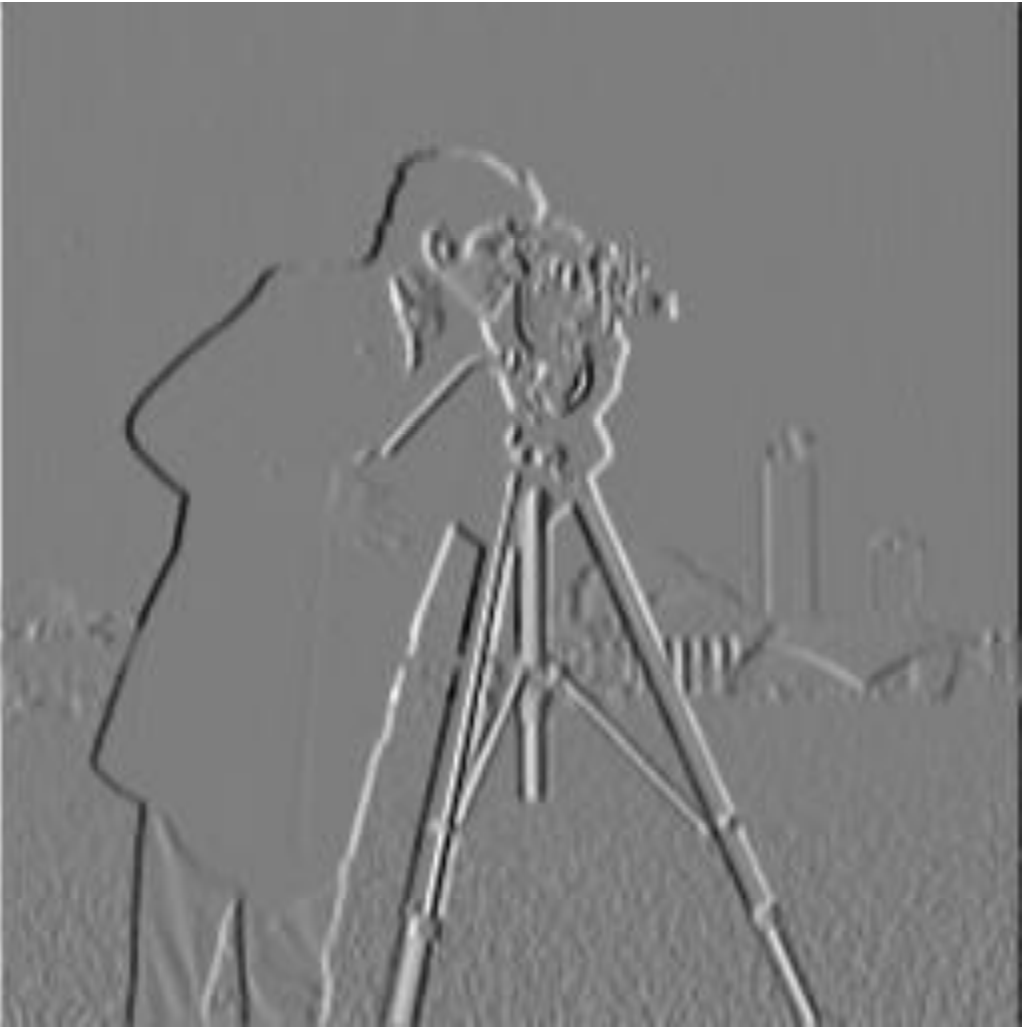
\includegraphics[width=\linewidth]{images/CameramanDx.png}
    \end{subfigure}
    \caption{Horizontal derivative with Sobel operator}
    \label{fig:Cameraman}
\end{figure}


In the DL field a Convolutional Neural Network is a NN that uses convolutional layers, usually to analyze images.
In a CNN the network is organized as a sequence of convolutional layers usually followed by few fully connected layers.
The sequence of convolutional layers learn the filters to be extracted directly from the input data; the layers extract features of increasing complexity as the layers progress from the input to the output layer.
Between convolutional layers it is common practice to use pooling layers. This is done to decrease the data dimensionality and be able to use more kernels to extract high level features.

\begin{figure}[h!]
    \centering
    \begin{subfigure}[]{0.4\linewidth}
        \label{fig:conv}
        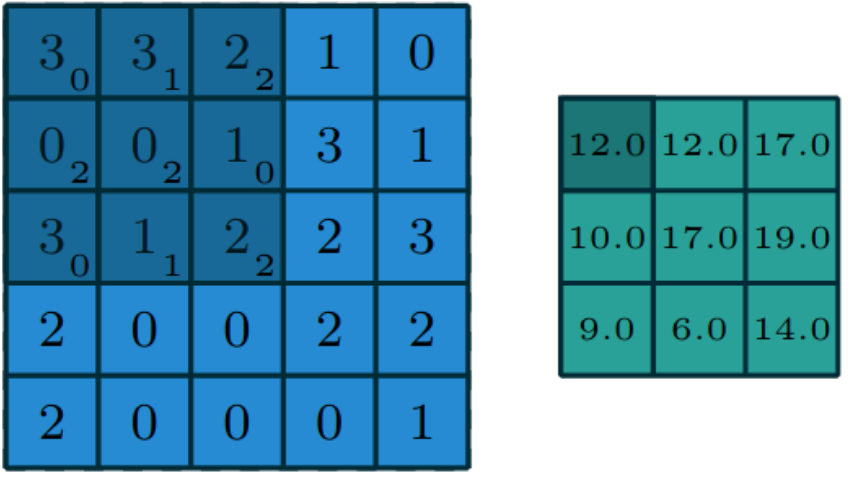
\includegraphics[width=\linewidth]{images/Convolution.png}
        \caption{2D Convolution}
    \end{subfigure}
    \hspace{1cm}
    \begin{subfigure}[]{0.4\linewidth}
        \label{fig:avgPool}
        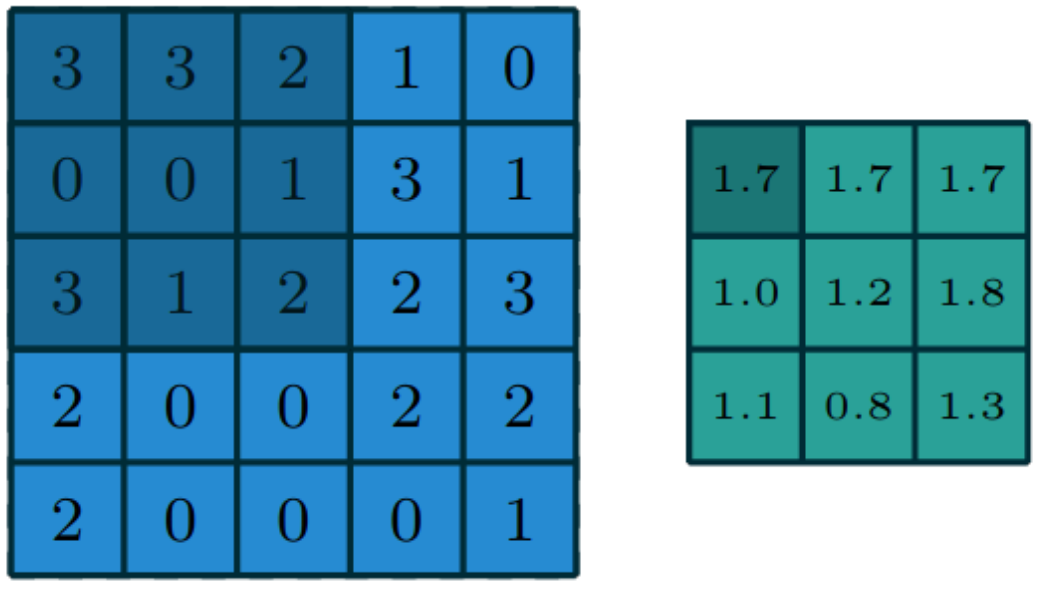
\includegraphics[width=\linewidth]{images/AVGPool.png}
        \caption{AVG Pool}
    \end{subfigure}
    \caption{Examples of 2D convolution (a) and AVG Pool operation (b). ~\cite{dumoulin2016guide}}
    \label{fig:ConvImgs}
\end{figure}

One interesting difference between how convolutions are tipically handled and how a CNN handle convolution is how they are performed on images with multiple channels.
The convolution operation is performed as usual but at the end all convolved channels are added pixelwise.
The number of channels of the output tensor is equal to the number of kernels considered by the convolution operation.

The CNN topology is inspired by how the animal visual cortex work; multiple neurons are connected in a hirearchical way to recognize features of increasing complexity. Neurons on the low level of the hirearchy recognize small features shuch as simple lines and corners; neurons at a higher levels recognize more abstract features such as more complex shapes and objects.

\begin{figure}[h!]
  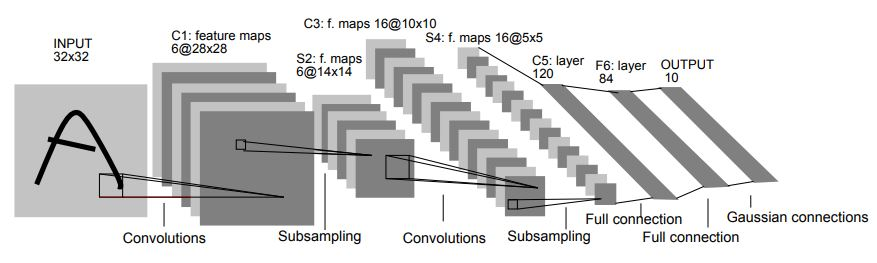
\includegraphics[width=0.9\textwidth]{images/lenet.jpg}
  \centering
  \caption{LeNet-5 architecture. Hand written digit recognition in 28x28 gray scale images. ~\cite{lenet}}
  \label{fig:lenet}
\end{figure}


\subsection{DL accelerators}

When a DL model must be deployed in a real system the forward pass can not always be done by simply using a CPU to perform the computation. The system is likely to have latency, throughput and power constraints that a simple CPU implementation is not able to deliver. CPUs have limited throughput performance and can exploit a limited ammount of coarse and fine grained parallelism.

Since the training phase uses batches of data to calculate the gradient for the next weight update GPGPUs are the most common choiche.
The high degree of parallelism that can be exploited from different weights and the different samples of the batch allow a GPU implmentation to exploit all the available parallelism.
In case of multiple GPUs available there are methods that allow to use all the available compuational power; multiple GPUs can be used to train bigger models with more parameters and use bigger batches to better approximate the true gradient.

Even if GPUs work great for parallelism when training a model they aren't always a good option when deploying a model.
GPUs are power hungry and since have a dedicated memory to perform computation they require time consuming memory transfers every time a kernel is executed.
This might be a problem, especially in latency constrained application where the system is required to process a stream of data where each sample depend on the decisions that the model has made at previous steps.

Multiple solutions are available to solve the problem of delivering high throughput and low latency while not exploiting the parallelism created by processing batches of data. The obvious and best possible solution to solve the problem would be to use specialized ASICs to perform the computation. This would deliver the best possible resoults in terms of final system performance but have its drawbacks. 
The long design time of specialized HW solutions is impractical in situations where fast propotyping is a desirable feature of the design process. 
Moreover ASIC solutions are not adaptable to new models, an ASIC would be usable only with a fixed subset of models and would not be able to adapt to future models using new and yet undiscovered layers.

A different and more adaptable solution while preserving the low latency and high troughput performances on streams of data is to use reconfigurable HW.
A possiblity is the use of FPGAs as deplyment targets.
FPGAs are configurable devices that incorporate logic and memory blocks; the configuration can be designed to implement the specific function that need to be computed by the specific application.
The use of FPGAs as targets allow the deployment on low level HW while being able to deploy different models by just reconfiguring the HW configuration \cite{DBLP:journals/corr/abs-1901-04988}.

An other advantage of FPGAs is the power efficency attainable; as long as the implementation manage properly the memory the use of FPGAs allow to maximize performance per watt.
An other big advantage of FPGAs over other solutions is the possibility of adapting the floating point precision of each operation to a degree that would not be possible with different HW solutions. 
The reconfigurability allow to implement operations whit a floating point precision with an arbitrary number of bits; the HW solution is not restricted to use a number of bits that is a power of 2. This lead to a more tailored implementation improving area utilization and buffer sizes.

The disadvantages of FPGA implementations are usually limited to a maximum buffer size and the long design time required to create a working and efficient implementation.
The long design time can be reduced by using High Level Synthesis tools that take as input a high level specification of the computation (as example the tool can take as input a filter written in C language) and output the bitstream ready to be deployed.

The result provided by a HLS tool do not have the same performance of a hand designed solution but the results are comparable. 
This also allow fast prototyping while enabling non HW experts to use specialized HW to deploy their trained models in real applications.

\section{ONNX}
\label{ONNX}

On the software side of the Deep Learning field multiple frameworks emerged to make easier for developers to create and train their models.
Since the DL field is realively new there is no established intermediate representation to optimize the abstract computational graph berfore producing the actual implementation; different frameworks use different representations designed to work only with one framework.

\begin{figure}[h!]
  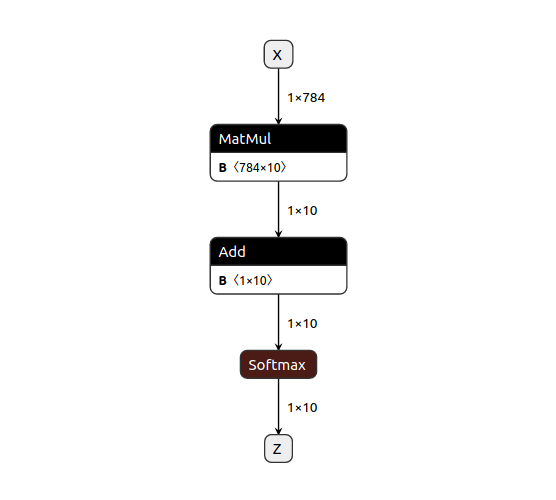
\includegraphics[width=0.9\textwidth]{images/ONNXExample.png}
  \centering
  \caption{Example of ONNX model.}
  \label{fig:onnx-example}
\end{figure}

The Open Neural Network eXchange (ONNX \cite{onnx}) has been created by Microsoft and Facebook with the goal of allowing the portability of computational graphs between different frameworks. 
The goal is to create an intermediate representation that can be used by different frameworks and be used to implement optimizations common to all frameworks.

The ONNX representation can also be used as common input representation for compilation stacks.
Since ONNX support the translation from computational graphs of main DL frameworks to a ONNX representation, the compilation stack can avoid the burden of implementing a different input procedure for each input DL framework and just rely on the ONNX standard.
ONNX is also likely to be maintained and if new and more recent frameworks are going to be developed the stack can rely on ONNX to provide a translation from the new computational graph to the already specified representation.

\section{Conclusions}
In this chapter we described the concepts necessary for the thesis. 
We described the main characteristics of Artificial Intelligence and what lead to the Machine Learning field.
The chapter also described Deep Learning models and how they are implemented in the context of image processing applications.
The next chapter is dedicated to the exploration of tools related to the contribution of the tesis.


\end{document}